\section{General Introduction}
Nowadays, with the rapid development of social networks, e-commerce, and sharing economies, it has become a core link of Internet services to discover users' needs, understand users' behaviors, and screen out the most relevant information and products for users. There is a huge amount of information on the Internet: YouTube users upload over 400 hours of video every minute; WeChat Moments receive 10 billion clicks per day; Instagram Stories have 500 million active users per day\footnote{Data sources: Instagram Revenue and Usage Statistics (2021).}. The recommendation system has become an essential part of various video websites and e-commerce websites to provide various personalized services for users to interact with the system.

Early recommendation systems relied more on simple models or algorithms guided by intuition. For example, the recommendation system based on information retrieval treats the user's information as a \textit{query} and baesd on various types of information to express the item to be recommended as a \textit{document}. Thus, the problem of recommending the most relevant set of items is transformed into the problem of finding the most relevant documents in information retrieval.
\begin{figure}[htbp]
\centering
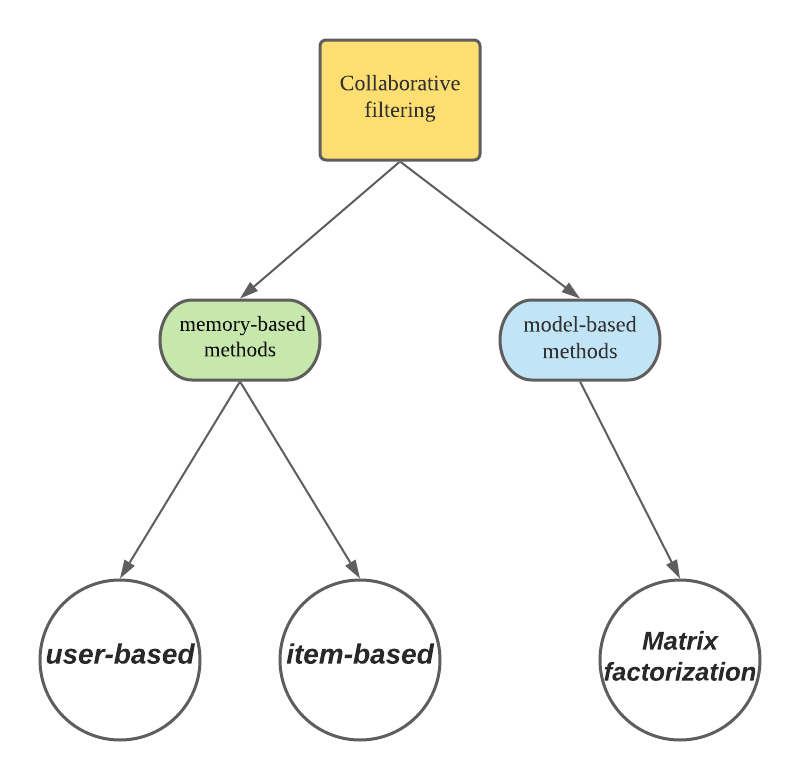
\includegraphics[scale=0.7]{figure/cfr.png}
\caption{Relation diagram of collaborative filtering in recommender systems}
\end{figure}
As the field of recommendation systems has evolved, traditional recommendation systems have been divided into two main categories: content-based filtering (CBF) and collaborative filtering (CF) \cite{cf1999}. The content-based approach describes the nature of users and items by defining explicit attributes (usually defined by experts with professional knowledge) and then recommends items that are \textit{``compatible"} with the user's nature. Traditional collaborative filtering, as shown in Figure 1.1, is categorized into two categories \cite{1423975}: memory-based methods and model-based methods. Item-based collaborative filtering and user-based collaborative filtering fall under the category of memory-based methods. For matrix factorization (MF), it is the most popular collaborative filtering technique that belongs to model-based methods \cite{convMF}.The three methods mentioned above will be elaborated and analyzed in the next chapter.

Matrix factorization attracts a ton of attention due to its good scalability and ease of implementation. In \cite{mf1}, the authors comprehensively introduce the matrix factorization algorithm, which integrates machine learning technology. Other than that, the authors in \cite{convMF} proposed a method that combines matrix factorization with convolutional neural networks (CNN). Matrix factorization is scalable; it can be seamlessly integrated with mainstream models and can also do feature fusion with multiple information sources. So, in \cite{mf2}, a model that fusion the text comment information, geographic neighborhood information, project category information, and popularity information has been proposed to promote the precision of rating prediction. However, these recommender systems focus on how to improve the accuracy of algorithms for a single problem (e.g., rating prediction for matrix factorization), thus neglecting the timeliness and systematicness of human-machine interaction, which makes it difficult to model the vagaries of user behavior and the rapidly changing external environment completely. These matrix factorization-based recommendation systems only exploit the trained model for the recommendation and do no proper exploration. Thus, these recommendation systems tend to produce cookie-cutter results.

In order to achieve a dynamic balance between the system and the user and to shift away from viewing the recommendation system as a running fragment of one recommendation result at a time. Some researchers, such as the authors in \cite{context} have started to explore how to apply some concepts of reinforcement learning to the scenario of recommendation systems. Reinforcement learning often represents a \textit{``feedback system"} in which the user and the system interact to achieve the optimization of the target. The interaction process between the system and users is no longer a \textit{``one-shot deal"}, which is replaced by the dynamic balance between the system and users that achieved through a series of results on the dimension of time.  A number of algorithms have been proposed based on the context-free bandit and the contextual bandit. Further detailed concepts and algorithms of context-free bandit and contextual bandit will be conducted in chapter 2.

However, in the more complex scenario of online mass recommendation systems, the above algorithm has not been favored. Although such algorithms have beautiful proofs and mathematical properties in theory, there are often insurmountable barriers to product experience in practice. As the authors affirm in \cite{conversation}, the contextual bandit algorithm requires a tremendous amount of exploration, resulting in a slow speed. Most of these algorithms are not familiar with the user in the initial period, so the algorithm tends to explore more items to understand the user. Therefore, during this period, the user may be confronted with a number of items that are not as relevant. In these algorithms, the assumption is that once the exploration period is over, the algorithm will be able to learn the user's preferences better and provide more \textit{``trustworthy"} recommendations. However, this hypothetical scenario does not hold in reality. In the real world, only highly loyal users may have the tolerance to accept less relevant recommendations. From the perspective of new users or users with low loyalty, the frequency of use of the product is not high, and when these users find some irrelevant recommendation results in a few uses, it is likely to cause new users to abandon the product permanently.

As alluded to above, collaborative filtering is the process of sifting and filtering information together with the relationship between users and their feedback on the items, to recommend items of interest to the target users. Since coordinated filtering focuses more on judging the similarity between historical records and a user’s similarity to make recommendations, the result is that the content universe of collaborative filtering is almost static and loses the ability to recommend new items. Unfortunately, in many recommendation scenarios, where the universe of content experiences rapid turnover and the popularity of content changes over time. Furthermore, the cold start \cite{cold} problem is also an insurmountable chasm for collaborative filtering.  In former research \cite{difficcf}, it was demonstrated that these problems led to poor performance and difficulty in applying traditional collaborative filtering-based recommender systems.

To address the aforementioned problems, in this work, BanditMF has been proposed, which is a multi-armed bandit based matrix factorization recommender system. This system combines the matrix factorization (MF) which is model-based collaborative filtering with the multi-armed bandit algorithm. BanditMF contains an offline subsystem focusing on matrix factorization and an online subsystem with a multi-armed bandit algorithm as its core. With the power of the multi-armed bandit algorithm, BanditMF solves the cold-start problem of the collaborative filtering method and gives the ability to recommend new items to users. Meanwhile, the bandit algorithm in the online subsystem accepts parameters from the matrix factorization in the offline subsystem to make recommendations. Since the matrix factorization takes into account the connections and similarities between users, the multi-armed bandit algorithm uses these parameters to reduce the irrelevance of the recommended items when exploring, thus reducing the loss of new users with low loyalty due to irrelevant recommendations from the bandit algorithm during the exploration period. The detailed discussion of BanditMF will be introduced in chapter 3.

The remainder of this report is organized as follows: In Chapter 2, the representative multi-armed bandit and collaborative filtering methods will be reviewed and formulated to solve the problem. In Chapter 3, two traditional systems will be illustrated: a collaborative filtering-based recommender system and a hybrid recommender system. Then, based on those traditional systems, BanditMF will be introduced in detail. In chapter 4, the two traditional systems are implemented and experimentally evaluated with BanditMF. We propose the future work and the conclusion of the entire work will be present in chapter 5.